%!TEX root = ../fbi.tex

\section{Construction of the featuresless boson insulator}

It was argued by Kimchi, et. al. \cite{kimchi2013} that this state represents a featureless Mott insulating phase of bosons on the honeycomb lattice.

\begin{equation}
\ket{\psi} = \prod\limits_{\varhexagon} \sum\limits_{i \in \varhexagon} b^{\dagger}_{i} \ket{0}
\label{eq:def}
\end{equation}

\begin{figure}[H]
	\centering
	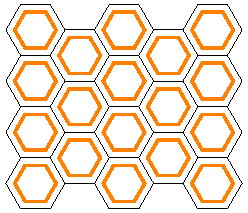
\includegraphics[width=0.6\columnwidth]{fbi3.pdf}
	\caption{Schematic representation of honeycomb FBI}
\end{figure}

\subsection{PEPS Construction of honeycomb F.B.I.}

With the local and translationally invariant description of the wavefunction in (\ref{eq:def}), we can construct a (translationally invariant) PEPS representation of $\ket{\psi}$ convenient for computations. 

The simplest example of a tensor network for a 1D system is a matrix product state; translationally-invariant matrix product states (MPS) are represented by a single rank 3 tensor $A_p^{ij}$ which specifies the wavefunction coefficients in a given basis local basis as a product of matrices $$\ket{\psi} = \sum\limits_{\{p_i\}} A_{p_1} A_{p_2} ... A_{p_N} \ket{p_0 p_1 ... p_N},$$
with one matrix for each site in the one-dimensional system.

\begin{figure}[H]
	\centering
	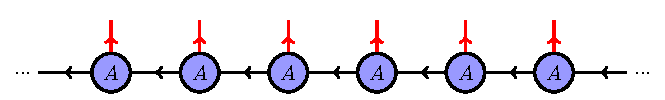
\includegraphics[width=\columnwidth]{mps.pdf}
	\caption{Pictoral representation of the tensor contraction for a matrix product state. Black lines are called virtual indices and are contracted over when computing wavefunction coefficients.}
	\label{fig:MPS}
\end{figure} 

PEPS are the generalization of MPS to two and higher dimensions, where each site in the system is represented by a rank $z+1$ tensor, where $z$ is the coordination number of the lattice, and wavefunction coefficients are similarly given by contracting over all virtual indices as shown in Figure \ref{fig:PEPS}.\cite{verstraete2004}

\begin{figure}[H]
	\centering
	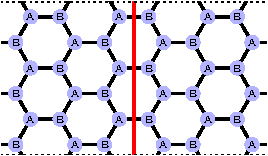
\includegraphics[width=\columnwidth]{Hex_PEPS.pdf}
	\caption{Pictoral representation of a PEPS on a honeycomb lattice. The tensors A and B are rank 4, with the physical leg at each site not shown for visual clarity. By gluing together the top and bottom edge of this picture, we get the "zig-zag" cylinder configuration used for most of the calculations in this paper. This cylinder is 3 unit cells wide, so we will call it the L=3 cylinder. In section \ref{sec:ES}, we will study the entanglement cut specified by the red line for various cylinder widths.}
	\label{fig:PEPS}
\end{figure}

We can represent (\ref{eq:def}) as a tensor network by replacing the sum over each plaquette with a tensor contraction. The matrix elements of the plaquette boson creation operator can be specfied by a trace over one virtual qubit per site $x$ adjacent to the plaquette, as in 
\begin{equation}
\braopket{\{\alpha_x\}}{\sum\limits_{x \in \varhexagon} b^{\dagger}_{x}}{\{\beta_x\}} =
 \sum\limits_{\{i_x\}} W^{i_1 i_2 ... i_6} \prod\limits_x B^{i_x}_{\alpha_x \beta_x} 
\label{eq:plaquette}
\end{equation}

in which the application of the creation operator at $x$ is controlled by the state of the virtual qubit $i_x$:

$$
B^i_{\alpha \beta} = \left\{
     \begin{array}{lr}
       \delta_{\alpha \beta} & : i = 0\\
       (b^{\dagger})_{\alpha \beta} & : i = 1
     \end{array}
   \right\}.
$$

The tensor $W^{i_0 i_1 i_2 i_3 i_4 i_5}$ should be taken as the W-state: 
$$ W^{\{i_x\}}  = \left\{ \begin{array}{lr}
													1  : & \sum\limits_x i_x = 1 \\
													0  : & \text{else}
													\end{array}
											\right\} = \ket{100000} + ...\ket{000001}.
$$

By applying the operator to all plaquettes, we get a tensor network not in the form of Figure \ref{fig:PEPS}, but instead one with the rank 6 tensor $W$ located on each plaquette and a rank $3+1$ tensor $D$ located on the vertices, as shown in \ref{fig:FBI_PEPS}. 

\begin{figure}[H]
	\centering
	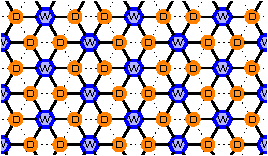
\includegraphics[width=0.8\columnwidth]{FBI_PEPS.pdf}
	\caption{Intermediate tensor network for F.B.I. state. The lines representing the physical indices exist on each vertex, but are suppressed in the picture for visual clarity.}
	\label{fig:FBI_PEPS}
\end{figure}

It is straightforward to show that the tensor $D^p_{ijk}$ should be
$$
D_{p}^{i_0 i_1 i_2} = \sum\limits_{\alpha \beta} B^{i_0}_{p \alpha}B^{i_1}_{\alpha \beta} B^{i_2}_{\beta 0}  = \left\{ \begin{array}{lr}
													\sqrt{p!}  : & p =i_0+i_1+i_2  \\
													0  : & \text{else}
													\end{array}
											\right\}
$$
to reproduce the action of the plaquette operators adjacent to each vertex. The boson number at the vertex $p$ can be limited to be $0, 1, 2,$ or $3$ since at most one boson comes from each of the three adjacent hexagons.

This tensor network wavefunction in this form manifestly has all the translational and point group symmetries of the honeycomb lattice, since the tensors $W$ and $D$ are invariant under rotations of their virtual indices in the plane, as shown in the picture. One can also check that the wavefunction is $U(1)$ invariant; all terms in the wavefunction are configurations with boson number exactly $1$ per plaquette.

In order to form a PEPS representation with all tensors located on the vertices, we can factor the W-state tensor and regroup the factors into PEPS tensors $A$ and $B$, as shown in Figure \ref{fig:FBI_PEPS_2}. 
There is a choice of MPS for the W-state that doesn't manifestly preserve the rotational symmetry the plaquettes, but has the small bond dimension $2$. (A different choice could be made that has bond dimension 6 but does preserve the symmetry.) This factorization of the W-state is given by

$$
W^{i_0 i_1 i_2 i_3 i_4 i_5} = \sum\limits_{abcde} W^{i_0 a}_{1} W^{i_1 b}_{a} W^{i_2 c}_{b} W^{i_3 d}_{c} W^{i_4 e}_{d} W^{i_5 0}_{e},
$$
where 
$$ W^{i_0 i_1}_{j}  = \left\{ \begin{array}{lr}
													1  : & i_0+i+1 = j \\
													0  : & \text{else}
													\end{array}
											\right\},
$$
and where each index takes values in $\{0, 1\}$. We will discover that the virtual edges in this PEPS can be assigned consistent $U(1)$ charges, with the index $i_x$ representing the charge. The arrows on the tensors show the flow of charge.

The rewriting of the tensor network does not change the physical wavefunction or physically invariant quantities, such as the Schmidt spectrum for the entanglement cut. However, it is computationally convenient - the total bond size crossed by the entanglement cut in Figure \ref{fig:PEPS} is $2^L$ for the cylinder of width $L$.

\begin{figure}[H]
	\centering
	\subfigure[W-state tensor and factored form]{%
		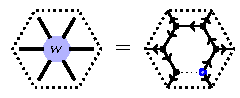
\includegraphics[width=0.6\columnwidth]{w_string.pdf}
		\label{fig:W}
	}
	\quad
	\subfigure[D tensor]{%
		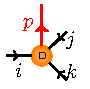
\includegraphics[width=0.3\columnwidth]{D_op.pdf}
		\label{fig:D}
	}
	\subfigure[PEPS tensor network for F.B.I. state]{%
		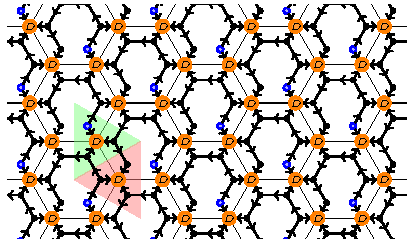
\includegraphics[width=0.8\columnwidth]{FBI_PEPS_2.pdf}
		\label{fig:FBI_PEPS_2A}
	}
		
%
\caption{Tensors used to put the F.B.I. tensor network in PEPS form. }
\label{fig:FBI_PEPS_2}
\end{figure}

%\begin{figure}[H]
%	\begin{columns}{t}
%	\begin{column}{width=0.25\textwidth]
%	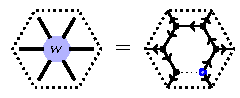
\includegraphics[width=0.6\columnwidth]{w_string.pdf}
%	\end{column}
%	\begin{column}{width=0.25\textwidth]
%	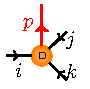
\includegraphics[width=0.6\columnwidth]{D_op.pdf}
%	\end{column}
%	\end{columns}
%\end{figure}
